% Appendix
\appendix
\section{Appendix}

\subsection{Omitted Proofs}

In this section the proofs that were omitted in the main part of the thesis are given.

\subsubsection{Eigenvalues of the Metric Matrix}
\label{proof_eigval}

\begin{proposition}
		Let \(A \in \R^{n\times n}\) a symmetric matrix, \(b \in \R\) and \(\mathbb{I} \in \R^{n\times n}\) the identity matrix.
		Let \(\lambda^A_i\), \(i = 1,...,n\) be the eigenvalues of the matrix \(A\). Then the eigenvalues of the matrix \(A+b\mathbb{I}\) are given by \(\tilde{\lambda}_i := \lambda^A_i + b\) for all \(i = 1,...,n\).
\end{proposition}

\begin{proof}
	Due to the symmetry of the matrix \(A\) it possesses  \(n\) real eigenvalues \(\lambda^A_i\).
	Let \(v^i\), \(i = 1,...,n\) be the corresponding eigenvectors. It follows that for \(i = 1,...,n\)
	
	\[ (A+b\mathbb{I})v^i = Av^i+bv^i = (\lambda_i^A + b)v^i. \]
	
	This means that \(v^i\) is an eigenvector of \(A+b\mathbb{I}\) to the eigenvalue \(\lambda_i^A + b\) for all \(i = 1,...,n\).
\end{proof}

\subsubsection{Proof of Proposition \ref{prop_norm}}
\label{proof_norm}

\begin{proof}
	We show that the scalar product \(\Langle x,y \Rangle_{Q_k+\frac{1}{t_k}\mathbb{I}} := x^{\top} (Q_k+\frac{1}{t_k}\mathbb{I})y\) is well-defined.
	This yields directly that also the norm induced by the scalar product is well-defined (see for example \cite[Corollary 12.6, p. 172]{Liesen2015}).
	
	By proposition \ref{prop_bounded} the matrix \(Q_k+\frac{1}{t_k}\mathbb{I}\) is bounded and relation (\ref{rel_bound}) assures that the following calculations are valid for all \(k\).
	
	We prove now that the matrix \(Q_k+\frac{1}{t_k}\mathbb{I}\) can be used to define a scalar product.
	
From the rules for matrix-vector multiplication follows that

\[ (x+y)^{\top}\left(Q_k+\frac{1}{t_k}\mathbb{I}\right)z = x^{\top}\left(Q_k+\frac{1}{t_k}\mathbb{I}\right)z + y^{\top}\left(Q_k+\frac{1}{t_k}\mathbb{I}\right)z, \quad x,y,z \in \R^n\]

and 

\[ x^{\top}\left(Q_k+\frac{1}{t_k}\mathbb{I}\right)(y+z) = x^{\top}\left(Q_k+\frac{1}{t_k}\mathbb{I}\right)y + x^{\top}\left(Q_k+\frac{1}{t_k}\mathbb{I}\right)z, \quad x,y,z \in \R^n.\]

Thus linearity of the defined scalar product is proven.

The symmetry of \(Q_k+\frac{1}{t_k}\mathbb{I}\) yields symmetry of the scalar product by

\[ x^{\top} \underbrace{\left(Q_k+\frac{1}{t_k}\mathbb{I}\right)y}_{:=\tilde{y}} = \tilde{y}^{\top}x = y^{\top}\left(Q_k+\frac{1}{t_k}\mathbb{I}\right)^{\top}x = y^{\top}\left(Q_k+\frac{1}{t_k}\mathbb{I}\right)x.   \]

Finally positive definiteness of the scalar product follows directly from positive definiteness of the matrix \(Q_k+\frac{1}{t_k}\mathbb{I}\).

This means the scalar product \(\langle \cdot,\cdot \rangle_{Q_k+\frac{1}{t_k}\mathbb{I}}\) is well defined and thus induces the norm \(\Vert \cdot \Vert_{Q_k+\frac{1}{t_k}\mathbb{I}}\).
\end{proof}

\subsection{Counterexaple to Strong Regularity}
\label{sec_counter_ex}
In section \ref{sec_SVMs} of this thesis it is claimed that problem (\ref{SVM_1}) may not be strongly regular at its solution.

It is remarked in \cite[p. 96]{Outrata1998} that if LICQ does not hold for a minimum \((w^{top},b,\xi^{top})\), then the GE coming from this problem is not strongly regular in this point.

In order to show that a situation where LICQ is violated in the minimum can be easily constructed, consider \(w \in \R^{n_f}\). In a usable machine learning problem the number of data points \(n_d\) is much larger than the size \(n_f\) of the feature space, in order to achieve reliable generalization.

Consider now, that \(n_f+2\) of the data points, that correspond to active constraints are correctly classified and sit directly on the margin. (This means, they are so called \emph{support vectors}. Refer to section 6.1.1 of \cite{Cristianini2000} for more information on this.)
For those points both of the constraints 

\[ y_i\left(\Langle w,x^i\Rangle-b\right) \geq 1-\xi_i \quad \text{and} \xi_i \geq 0 \]

hold with equality.

This means, that by renumbering these constraints the matrix with the derivatives of them has the following form:

\[  \tilde{A} = \begin{pmatrix} -y_1(x^1)^{\top} & 1 & -1 \\
                     \vdots & \vdots & & \ddots \\
										-y_{n_f+2}(x^{n_f+2})^{\top} & 1 & & & -1\\										0 & 0 & -1 \\
										\vdots & \vdots & & \ddots \\
										0 & 0 & & & -1\end{pmatrix}.\]
										
As it was assumed that there are \(n_f+2\) such data points, this matrix cannot have linearly independent rows. This means that LICQ does not hold in the given solution and therefore also strong regularity is violated.

\subsection{Additional Figures}

\subsubsection{Variable Metric Bundle Method}

The following plots show the behavior in accuracy and number of steps of the proximal bundle algorithm \ref{sec_nonconv_inex}.1 and different realizations of the variable metric bundle method \ref{sec_variable_metric}.1 when optimizing the Ferrier polynomials \(f_1\) to \(f_5\) in different dimensions and for different noise forms.
The conditions and parameters used for the plots are described in section \ref{sec_num_test_ferr}

The two plots below depict the situation for \(x \in \R^n\) for \(n = 2,3,...,15\).

\begin{figure}[H]
	\begin{subfigure}{0.49\textwidth}
		%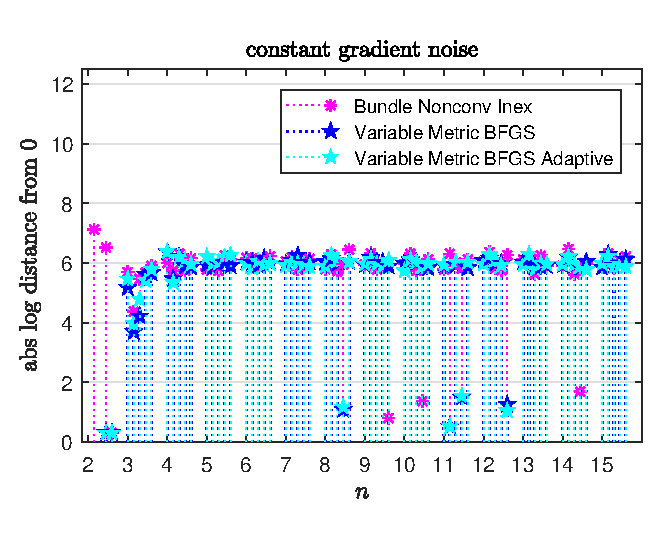
\includegraphics[width=\textwidth]{Pictures/Plots/constant_gradient_noise.eps}%
	\end{subfigure}
	\begin{subfigure}{0.49\textwidth}
		%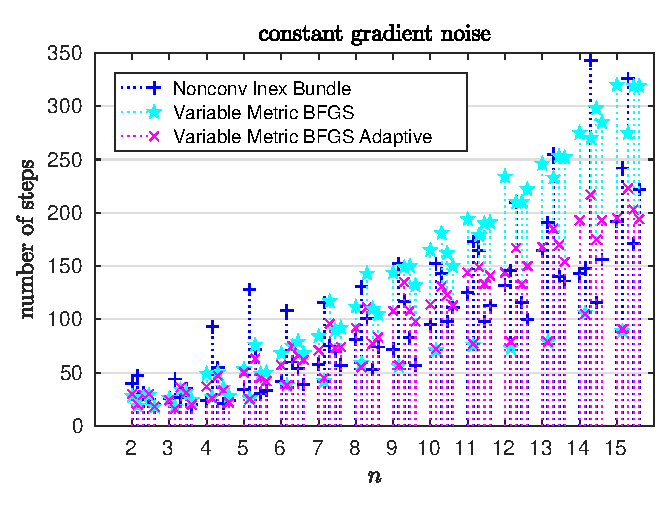
\includegraphics[width=\textwidth]{Pictures/Plots/steps_constant_gradient_noise.eps}%
	\end{subfigure}
	\caption[Accuracy and number of steps for: constant gradient noise]{Comparison of accuracy and number of steps for the proximal bundle algorithm and the variable metric bundle algorithm in the case of constant gradient noise}%
	\label{fig_const_grad_noise}%
\end{figure}

\vspace{-1.5em}

\begin{figure}[H]
	\begin{subfigure}{0.49\textwidth}
		%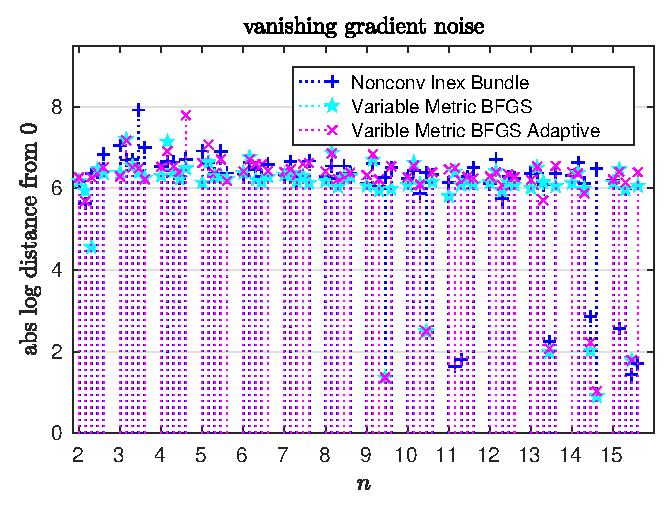
\includegraphics[width=\textwidth]{Pictures/Plots/vanishing_gradient_noise.eps}%
	\end{subfigure}
	\begin{subfigure}{0.49\textwidth}
		%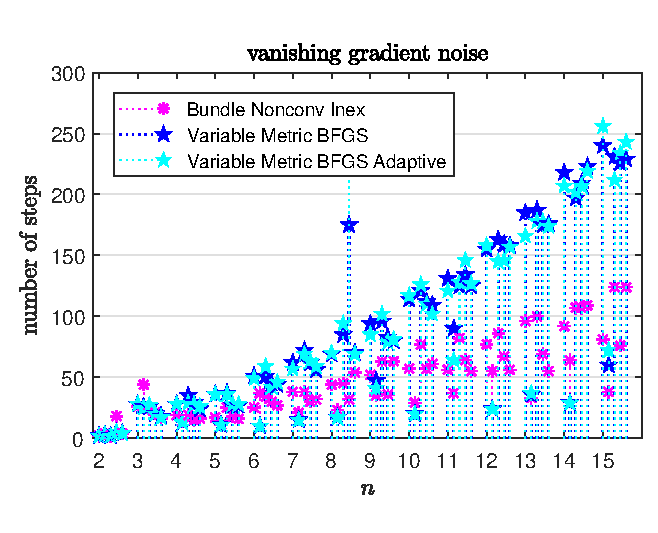
\includegraphics[width=\textwidth]{Pictures/Plots/steps_vanishing_gradient_noise.eps}%
	\end{subfigure}
	\caption[Accuracy and number of steps: vanishing gradient noise]{Comparison of accuracy and number of steps for the proximal bundle algorithm and the variable metric bundle algorithm in the case of vanishing gradient noise}%
	\label{fig_van_grad_noise}%
\end{figure}


The following plots show the situation for larger dimensions \(n = \{20,25,30,40,50\}\).


\begin{figure}[H]%
	\begin{subfigure}{0.49\textwidth}
		%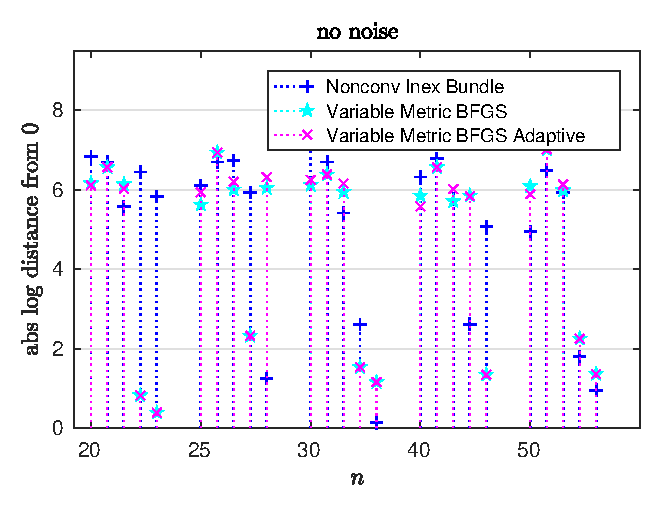
\includegraphics[width=\textwidth]{Pictures/Plots/no_noise_b.eps}%
	\end{subfigure}
	\begin{subfigure}{0.49\textwidth}
		%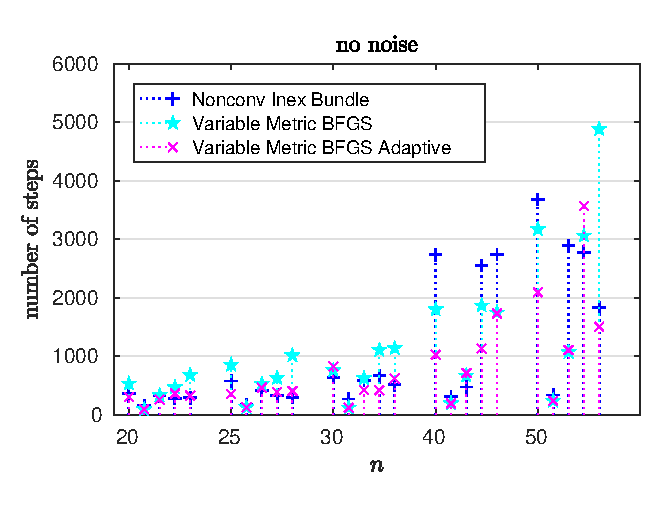
\includegraphics[width=\textwidth]{Pictures/Plots/steps_no_noise_b.eps}%
	\end{subfigure}
	\caption[Accuracy and number of steps: no noise, higher dimensions]{Comparison of accuracy and number of steps for the proximal bundle algorithm and the variable metric bundle algorithm in the case of no noise}
	\label{fig_no_noise_large}

\end{figure}

\vspace{-1.5em}

\begin{figure}[H]
	\begin{subfigure}{0.49\textwidth}
		%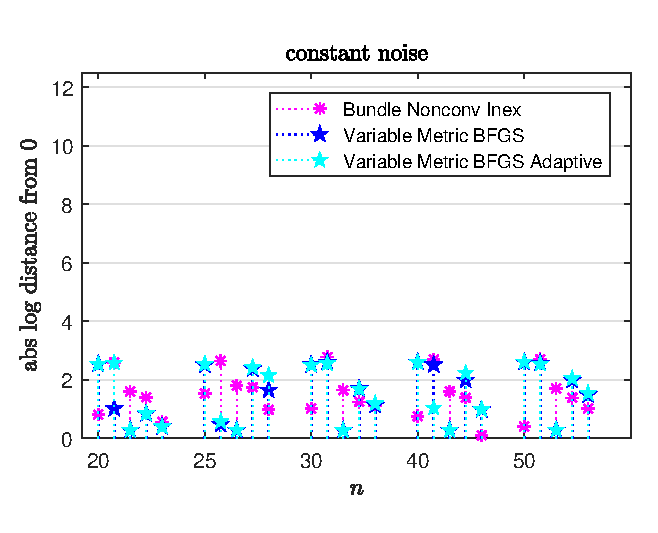
\includegraphics[width=\textwidth]{Pictures/Plots/constant_noise_b.eps}%
	\end{subfigure}
	\begin{subfigure}{0.49\textwidth}
		%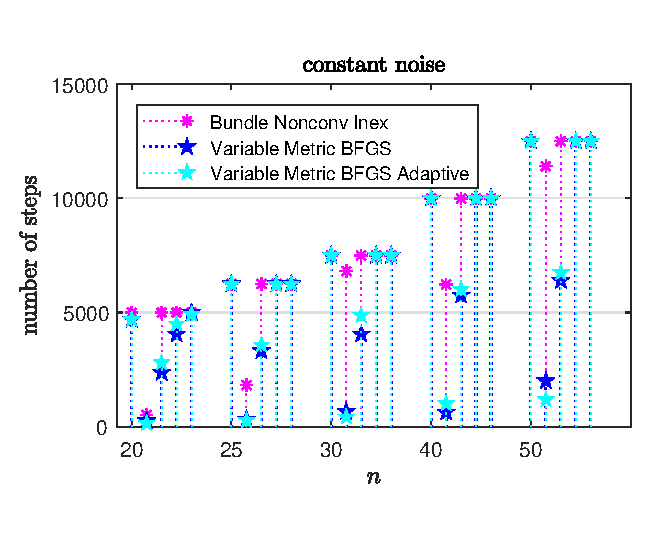
\includegraphics[width=\textwidth]{Pictures/Plots/steps_constant_noise_b.eps}%
	\end{subfigure}
	\vspace{-.5em}
	\caption[Accuracy and number of steps:constant noise, higher dimensions]{Comparison of accuracy and number of steps for the proximal bundle algorithm and the variable metric bundle algorithm in the case of constant noise}%
	\label{fig_const_noise_large}%
\end{figure}

\vspace{-1.5em}

\begin{figure}[H]
	\begin{subfigure}{0.49\textwidth}
		%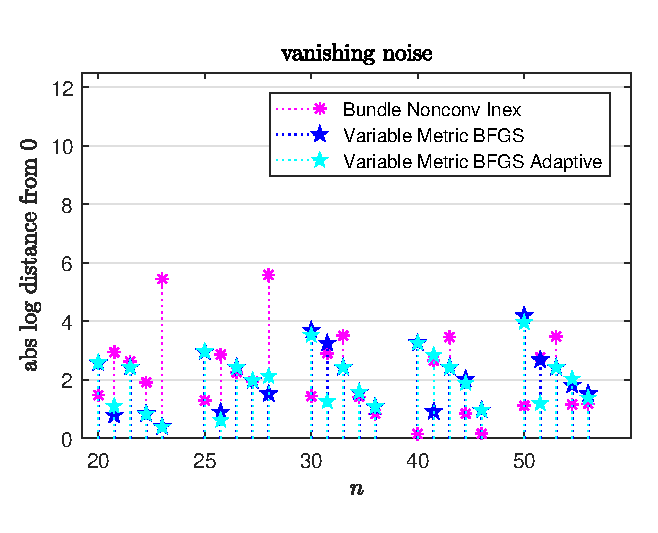
\includegraphics[width=\textwidth]{Pictures/Plots/vanishing_noise_b.eps}%
	\end{subfigure}
	\begin{subfigure}{0.49\textwidth}
		%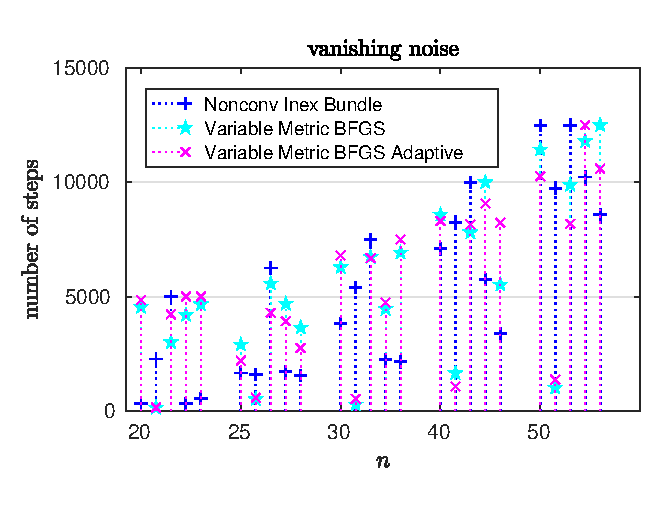
\includegraphics[width=\textwidth]{Pictures/Plots/steps_vanishing_noise_b.eps}%
	\end{subfigure}
	\caption[Accuracy and number of steps: vanishing noise, higher dimensions]{Comparison of accuracy and number of steps for the proximal bundle algorithm and the variable metric bundle algorithm in the case of vanishing noise}%
	\label{fig_van_noise_large}%
\end{figure}

\vspace{-1.5em}

\begin{figure}[H]
	\begin{subfigure}{0.49\textwidth}
		%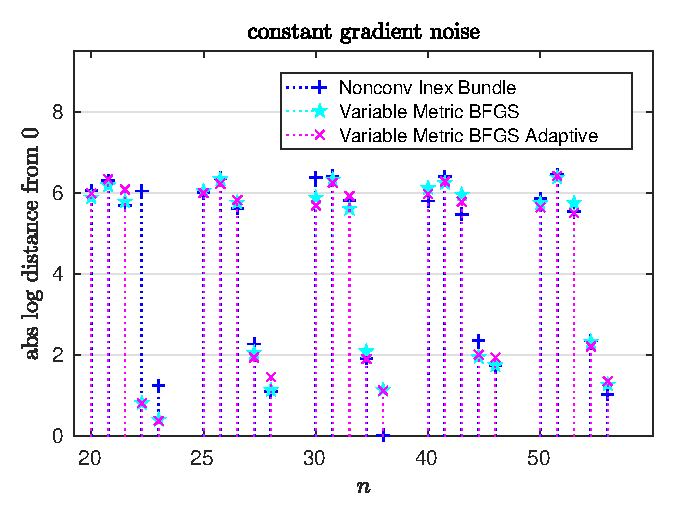
\includegraphics[width=\textwidth]{Pictures/Plots/constant_gradient_noise_b.eps}%
	\end{subfigure}
	\begin{subfigure}{0.49\textwidth}
		%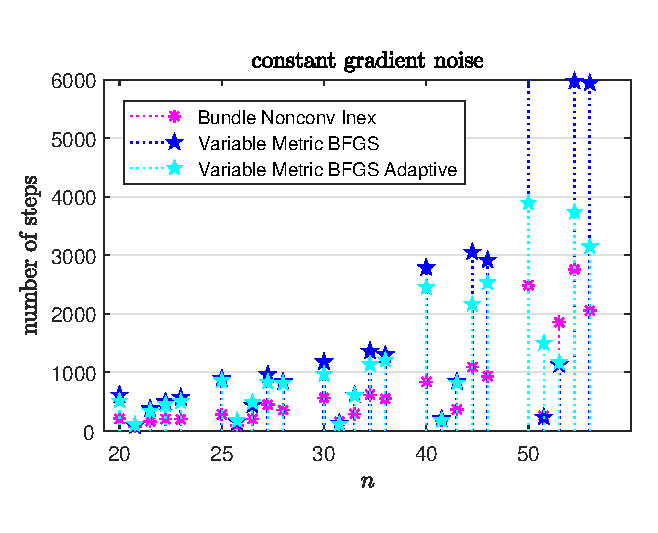
\includegraphics[width=\textwidth]{Pictures/Plots/steps_constant_gradient_noise_b.eps}%
	\end{subfigure}
	\caption[Accuracy and number of steps: constant gradient noise, higher dimensions]{Comparison of accuracy and number of steps for the proximal bundle algorithm and the variable metric bundle algorithm in the case of constant gradient noise}%
	\label{fig_const_grad_noise_large}%
\end{figure}

\vspace{-1.5em}

\begin{figure}[H]
	\begin{subfigure}{0.49\textwidth}
		%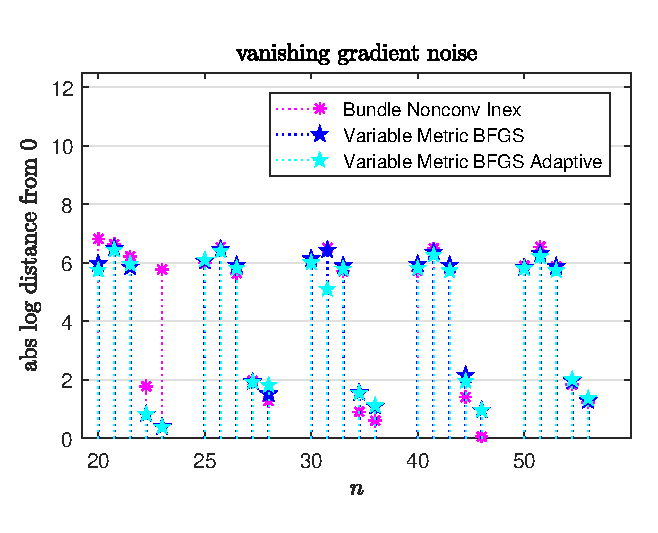
\includegraphics[width=\textwidth]{Pictures/Plots/vanishing_gradient_noise_b.eps}%
	\end{subfigure}
	\begin{subfigure}{0.49\textwidth}
		%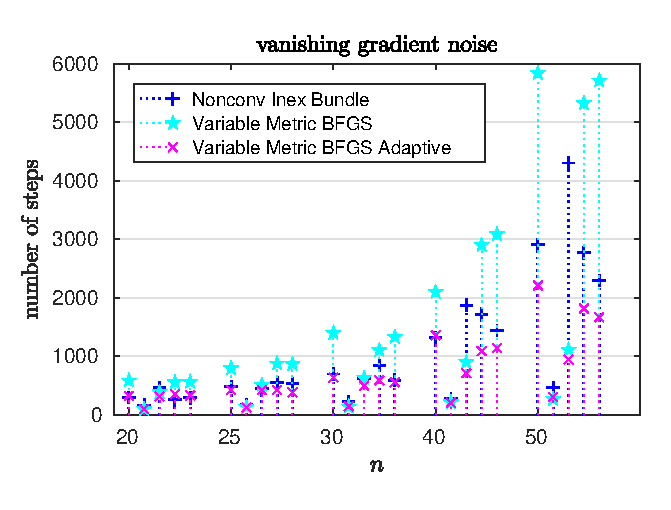
\includegraphics[width=\textwidth]{Pictures/Plots/steps_vanishing_gradient_noise_b.eps}%
	\end{subfigure}
	\caption[Accuracy and number of steps: vanishing gradient noise, higher dimensions]{Comparison of accuracy and number of steps for the proximal bundle algorithm and the variable metric bundle algorithm in the case of vanishing gradient noise}%
	\label{fig_van_grad_noise_large}%
\end{figure}

Next come the figures that illustrate the difference in behavior for different step size updating parameter \(\kappa_+\) and the performance of the hybrid method. In this method the metric matrix is scaled for boundedness of the eigenvalues and then scaled again by \(1/k\).


%\begin{figure}[H]
	%\begin{subfigure}{0.49\textwidth}
		%%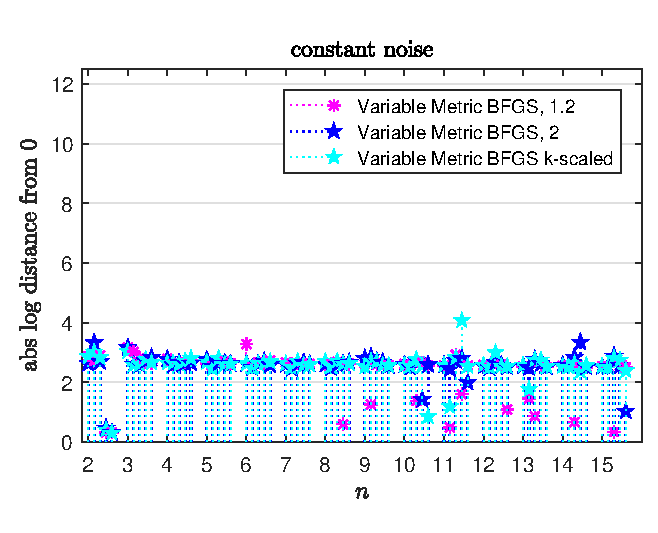
\includegraphics[width=\textwidth]{Pictures/Plots/constant_noise_comp.eps}%
	%\end{subfigure}
	%\begin{subfigure}{0.49\textwidth}
		%%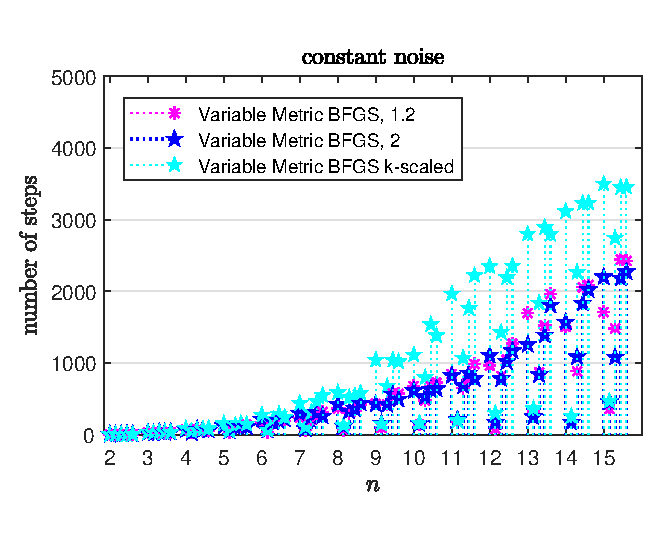
\includegraphics[width=\textwidth]{Pictures/Plots/steps_constant_noise_comp.eps}%
	%\end{subfigure}
	%\caption{Influence of the step size updating parameter \(\kappa_+ = 1.2\) and \(\kappa_+ =2 \) and performance of the hybrid method for constant noise. The reached accuracy is depicted on the left, the needed number of steps on the right.}%
	%\label{fig_const_noise_comp}%
%\end{figure}
%
%\vspace{-1.5em}

\begin{figure}[H]
	\begin{subfigure}{0.49\textwidth}
		%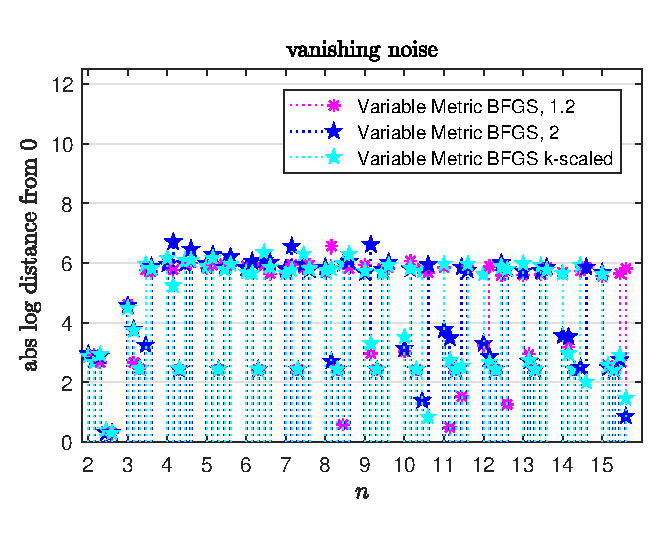
\includegraphics[width=\textwidth]{Pictures/Plots/vanishing_noise_comp.eps}%
	\end{subfigure}
	\begin{subfigure}{0.49\textwidth}
		%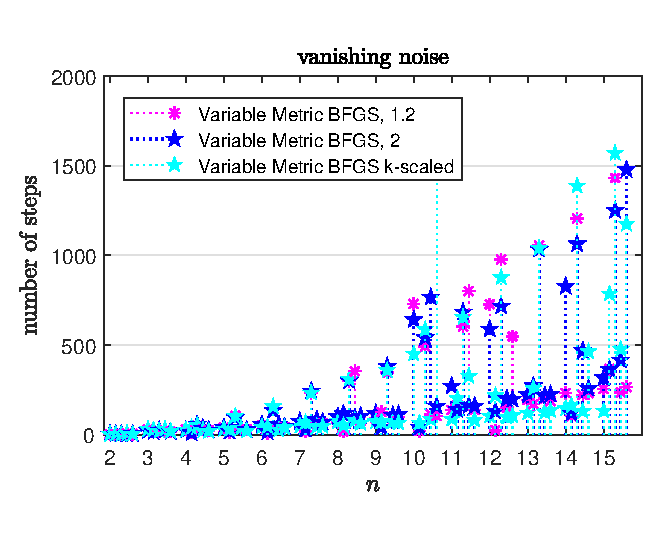
\includegraphics[width=\textwidth]{Pictures/Plots/steps_vanishing_noise_comp.eps}%
	\end{subfigure}
	\caption[Influence of the step size updating parameter and hybrid method: vanishing noise]{Influence of the step size updating parameter \(\kappa_+ = 1.2\) and \(\kappa_+ =2 \) and performance of the hybrid method for vanishing noise.}%
	\label{fig_van_noise_comp}%
\end{figure}

\vspace{-1.5em}

\begin{figure}[H]
	\begin{subfigure}{0.49\textwidth}
		%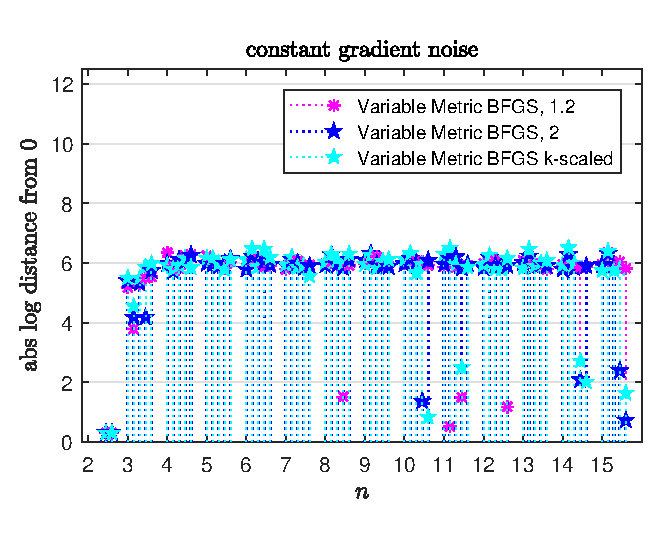
\includegraphics[width=\textwidth]{Pictures/Plots/constant_gradient_noise_comp.eps}%
	\end{subfigure}
	\begin{subfigure}{0.49\textwidth}
		%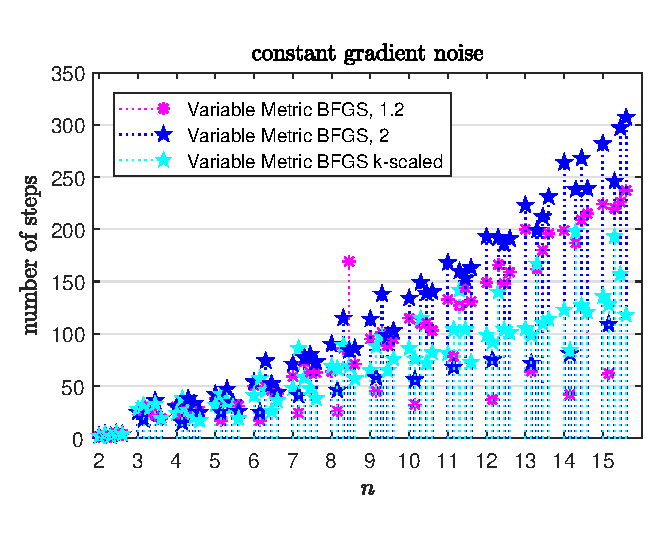
\includegraphics[width=\textwidth]{Pictures/Plots/steps_constant_gradient_noise_comp.eps}%
	\end{subfigure}
	\caption[Influence of the step size updating parameter and hybrid method: constant gradient noise]{Influence of the step size updating parameter \(\kappa_+ = 1.2\) and \(\kappa_+ =2 \) and performance of the hybrid method for constant gradient noise.}%
	\label{fig_const_grad_noise_comp}%
\end{figure}

\vspace{-1.5em}

\begin{figure}[H]
	\begin{subfigure}{0.49\textwidth}
		%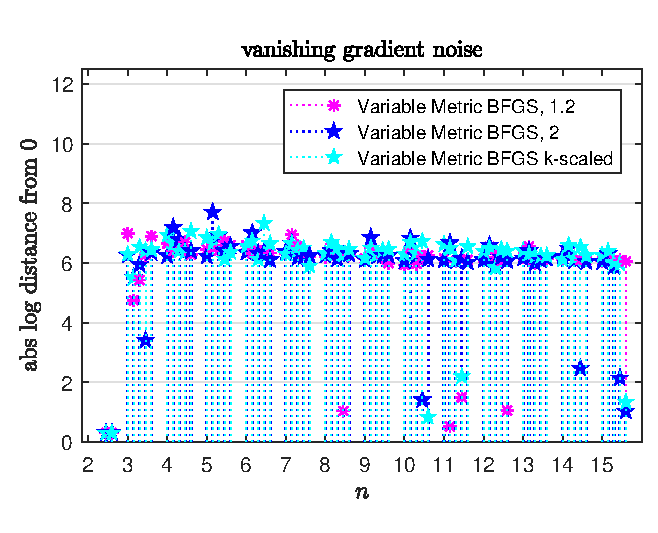
\includegraphics[width=\textwidth]{Pictures/Plots/vanishing_gradient_noise_comp.eps}%
	\end{subfigure}
	\begin{subfigure}{0.49\textwidth}
		%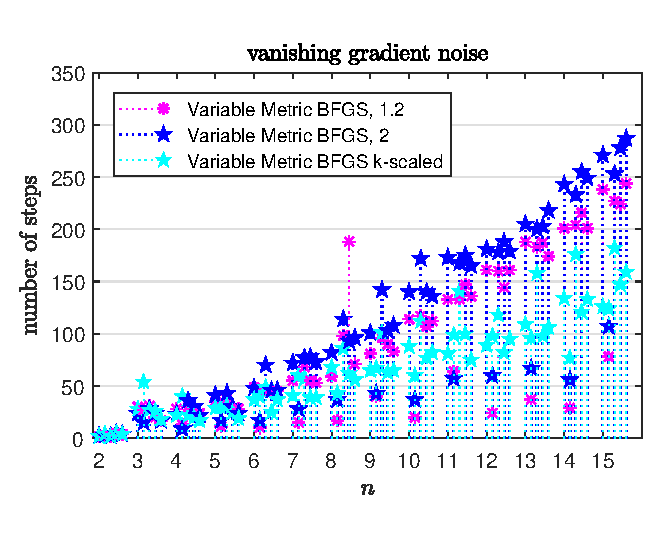
\includegraphics[width=\textwidth]{Pictures/Plots/steps_vanishing_gradient_noise_comp.eps}%
	\end{subfigure}
	\caption[Influence of the step size updating parameter and hybrid method: vanishing gradient noise]{Influence of the step size updating parameter \(\kappa_+ = 1.2\) and \(\kappa_+ =2 \) and performance of the hybrid method for vanishing gradient noise.}%
	\label{fig_van_grad_noise_comp}%
\end{figure}

\vspace{-1.5em}


%Following plots are in Noll part with \(\kappa_+ = 1.2, 2\) and in \(1/k\) part with \(\kappa_+ = 1.2\) for the large dimension
\begin{figure}[H]%
	\begin{subfigure}{0.49\textwidth}
		%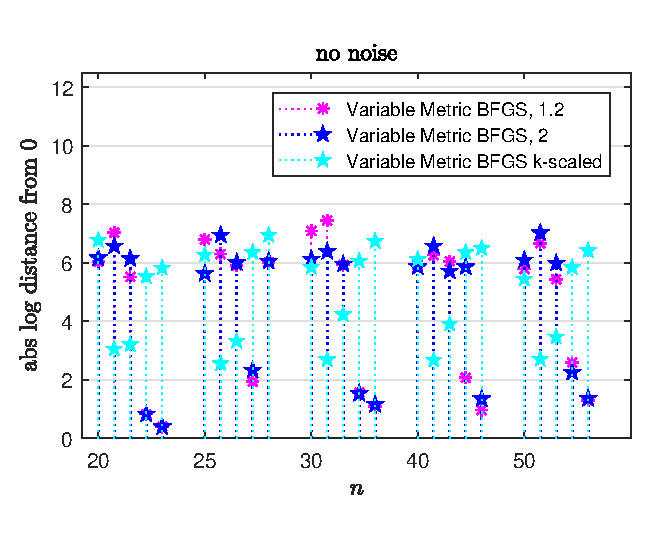
\includegraphics[width=\textwidth]{Pictures/Plots/no_noise_compb.eps}%
	\end{subfigure}
	\begin{subfigure}{0.49\textwidth}
		%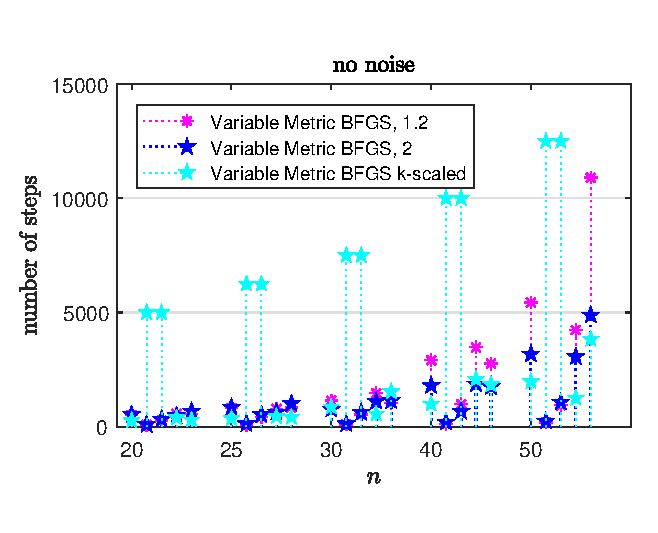
\includegraphics[width=\textwidth]{Pictures/Plots/steps_no_noise_compb.eps}%
	\end{subfigure}
	\label{fig_no_noise_comp_large}
	\caption[Influence of the step size updating parameter and hybrid method: vanishing noise, higher dimensions]{Influence of the step size updating parameter \(\kappa_+ = 1.2\) and \(\kappa_+ =2 \) and performance of the hybrid method for the exact case for higher \(x\)-dimensions. The reached accuracy is depicted on the left, the needed number of steps on the right.}
\end{figure}

\vspace{-1.5em}

\begin{figure}[H]
	\begin{subfigure}{0.49\textwidth}
		%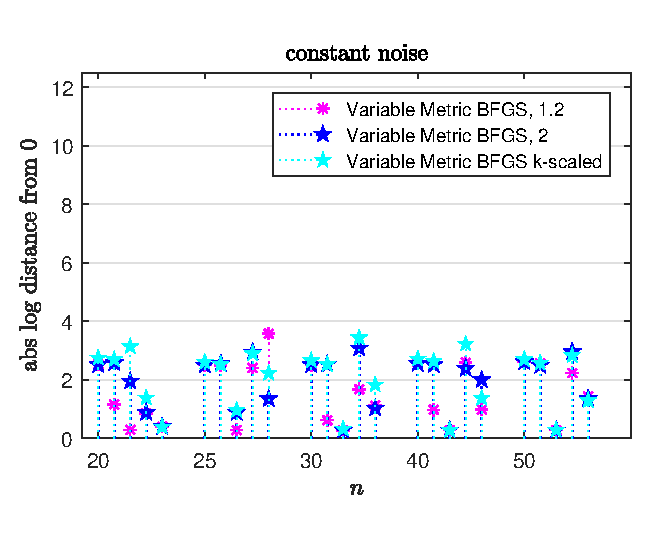
\includegraphics[width=\textwidth]{Pictures/Plots/constant_noise_compb.eps}%
	\end{subfigure}
	\begin{subfigure}{0.49\textwidth}
		%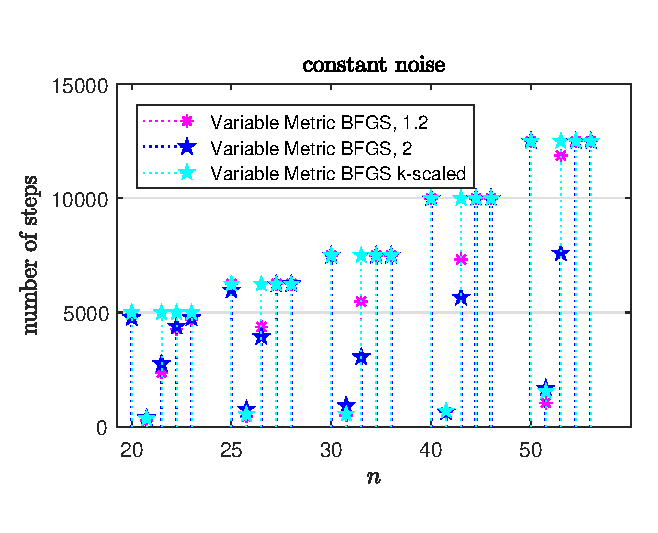
\includegraphics[width=\textwidth]{Pictures/Plots/steps_constant_noise_compb.eps}%
	\end{subfigure}
	\caption[Influence of the step size updating parameter and hybrid method: constant noise, higher dimensions]{Influence of the step size updating parameter \(\kappa_+ = 1.2\) and \(\kappa_+ =2 \) and performance of the hybrid method for constant noise.}%
	\label{fig_const_noise_comp_large}%
\end{figure}

\vspace{-1.5em}

\begin{figure}[H]
	\begin{subfigure}{0.49\textwidth}
		%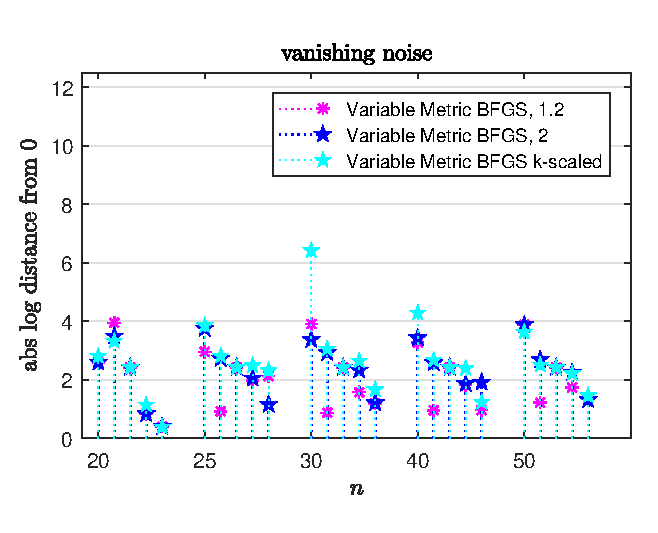
\includegraphics[width=\textwidth]{Pictures/Plots/vanishing_noise_compb.eps}%
	\end{subfigure}
	\begin{subfigure}{0.49\textwidth}
		%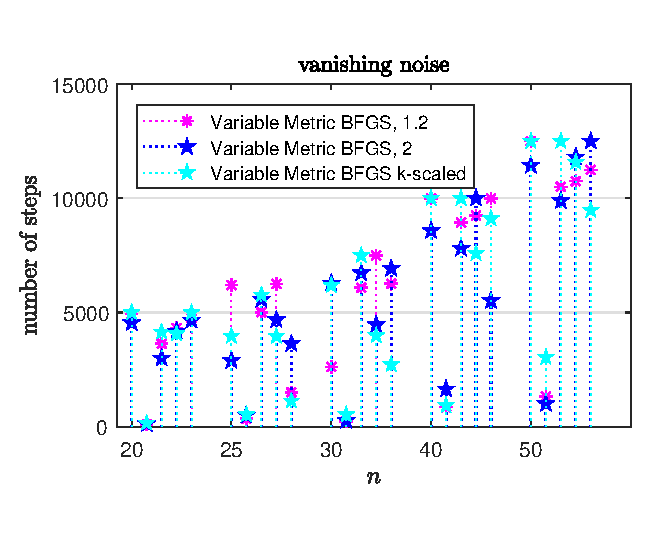
\includegraphics[width=\textwidth]{Pictures/Plots/steps_vanishing_noise_compb.eps}%
	\end{subfigure}
	\caption[Influence of the step size updating parameter and hybrid method: vanishing noise, higher dimensions]{Influence of the step size updating parameter \(\kappa_+ = 1.2\) and \(\kappa_+ =2 \) and performance of the hybrid method for vanishing noise.}%
	\label{fig_van_noise_comp_large}%
\end{figure}

\vspace{-1.5em}

\begin{figure}[H]
	\begin{subfigure}{0.49\textwidth}
		%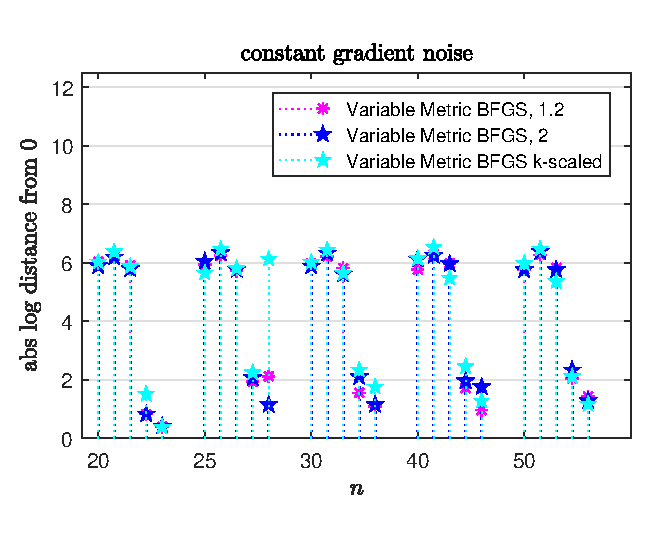
\includegraphics[width=\textwidth]{Pictures/Plots/constant_gradient_noise_compb.eps}%
	\end{subfigure}
	\begin{subfigure}{0.49\textwidth}
		%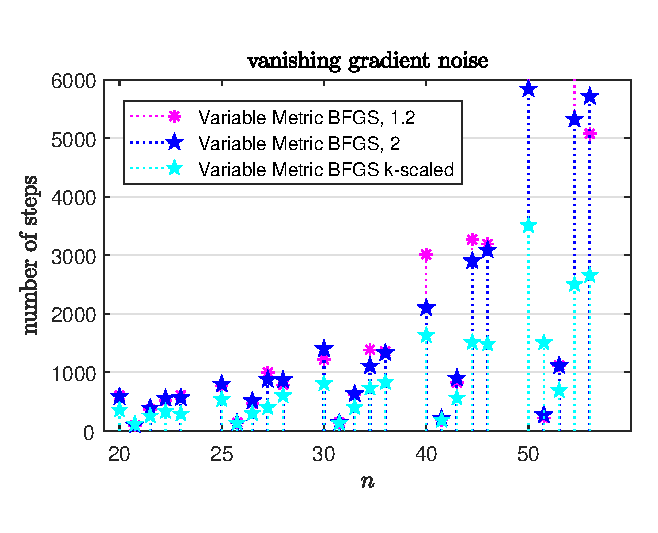
\includegraphics[width=\textwidth]{Pictures/Plots/steps_constant_gradient_noise_compb.eps}%
	\end{subfigure}
	\caption[Influence of the step size updating parameter and hybrid method: constant gradient noise, higher dimensions]{Influence of the step size updating parameter \(\kappa_+ = 1.2\) and \(\kappa_+ =2 \) and performance of the hybrid method for constant gradient noise.}%
	\label{fig_const_grad_noise_comp_large}%
\end{figure}

\vspace{-1.5em}

\begin{figure}[H]
	\begin{subfigure}{0.49\textwidth}
		%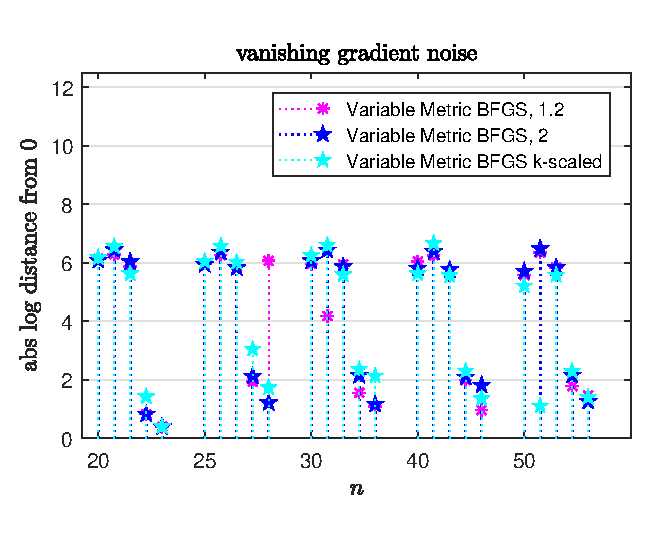
\includegraphics[width=\textwidth]{Pictures/Plots/vanishing_gradient_noise_compb.eps}%
	\end{subfigure}
	\begin{subfigure}{0.49\textwidth}
		%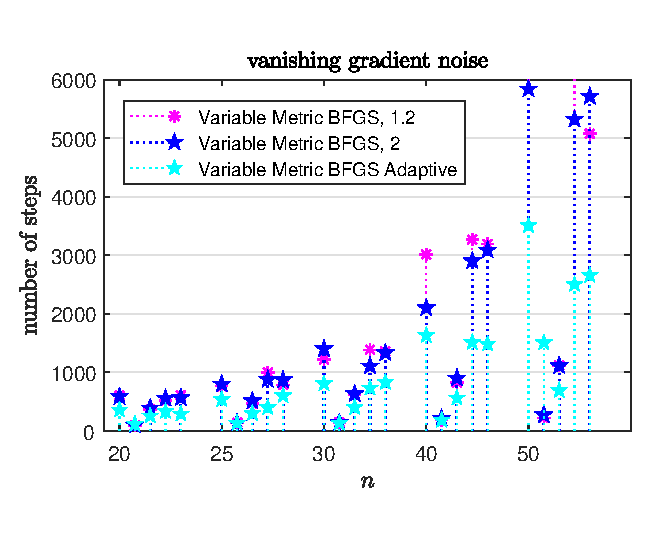
\includegraphics[width=\textwidth]{Pictures/Plots/steps_vanishing_gradient_noise_compb.eps}%
	\end{subfigure}
	\caption[Influence of the step size updating parameter and hybrid method: vanishing gradient noise, higher dimensions]{Influence of the step size updating parameter \(\kappa_+ = 1.2\) and \(\kappa_+ =2 \) and performance of the hybrid method for vanishing gradient noise.}%
	\label{fig_van_grad_noise_comp_large}%
\end{figure}

